%%%%%%%%%%%%%%%%%%%%%%%%%%%%%%%%%%%%%%%%%%%%%%%%%%%%%%%%%%%%%%%%%%%%%
%% This is a (brief) model paper using the achemso class
%% The document class accepts keyval options, which should include
%% the target journal and optionally the manuscript type. 
%%%%%%%%%%%%%%%%%%%%%%%%%%%%%%%%%%%%%%%%%%%%%%%%%%%%%%%%%%%%%%%%%%%%%
\documentclass[journal=jacsat,manuscript=article]{achemso}

%%%%%%%%%%%%%%%%%%%%%%%%%%%%%%%%%%%%%%%%%%%%%%%%%%%%%%%%%%%%%%%%%%%%%
%% Place any additional packages needed here.  Only include packages
%% which are essential, to avoid problems later. Do NOT use any
%% packages which require e-TeX (for example etoolbox): the e-TeX
%% extensions are not currently available on the ACS conversion
%% servers.
%%%%%%%%%%%%%%%%%%%%%%%%%%%%%%%%%%%%%%%%%%%%%%%%%%%%%%%%%%%%%%%%%%%%%
\usepackage[version=3]{mhchem} % Formula subscripts using \ce{}

%%%%%%%%%%%%%%%%%%%%%%%%%%%%%%%%%%%%%%%%%%%%%%%%%%%%%%%%%%%%%%%%%%%%%
%% If issues arise when submitting your manuscript, you may want to
%% un-comment the next line.  This provides information on the
%% version of every file you have used.
%%%%%%%%%%%%%%%%%%%%%%%%%%%%%%%%%%%%%%%%%%%%%%%%%%%%%%%%%%%%%%%%%%%%%
%%\listfiles

%%%%%%%%%%%%%%%%%%%%%%%%%%%%%%%%%%%%%%%%%%%%%%%%%%%%%%%%%%%%%%%%%%%%%
%% Place any additional macros here.  Please use \newcommand* where
%% possible, and avoid layout-changing macros (which are not used
%% when typesetting).
%%%%%%%%%%%%%%%%%%%%%%%%%%%%%%%%%%%%%%%%%%%%%%%%%%%%%%%%%%%%%%%%%%%%%
\newcommand*\mycommand[1]{\texttt{\emph{#1}}}

%%%%%%%%%%%%%%%%%%%%%%%%%%%%%%%%%%%%%%%%%%%%%%%%%%%%%%%%%%%%%%%%%%%%%
%% Meta-data block
%% ---------------
%% Each author should be given as a separate \author command.
%%
%% Corresponding authors should have an e-mail given after the author
%% name as an \email command. Phone and fax numbers can be given
%% using \phone and \fax, respectively; this information is optional.
%%
%% The affiliation of authors is given after the authors; each
%% \affiliation command applies to all preceding authors not already
%% assigned an affiliation.
%%
%% The affiliation takes an option argument for the short name.  This
%% will typically be something like "University of Somewhere".
%%
%% The \altaffiliation macro should be used for new address, etc.
%% On the other hand, \alsoaffiliation is used on a per author basis
%% when authors are associated with multiple institutions.
%%%%%%%%%%%%%%%%%%%%%%%%%%%%%%%%%%%%%%%%%%%%%%%%%%%%%%%%%%%%%%%%%%%%%
\author{Sélène Forget}
\affiliation[ENS]
{CPCV, Département de Chimie, École Normale Supérieure, PSL University, Sorbonne University, CNRS, 75005 Paris}
\email{selene.forget@ens.psl.eu}
\author{I. Ken Groupleader}
\email{guillaume.stirnemann@ens.psl.eu}
\affiliation[ENS]
{CPCV, Département de Chimie, École Normale Supérieure, PSL University, Sorbonne University, CNRS, 75005 Paris}

%%%%%%%%%%%%%%%%%%%%%%%%%%%%%%%%%%%%%%%%%%%%%%%%%%%%%%%%%%%%%%%%%%%%%
%% The document title should be given as usual. Some journals require
%% a running title from the author: this should be supplied as an
%% optional argument to \title.
%%%%%%%%%%%%%%%%%%%%%%%%%%%%%%%%%%%%%%%%%%%%%%%%%%%%%%%%%%%%%%%%%%%%%
\title[An \textsf{achemso} demo]
  {Molecular Dissection of Hairpin Ribozyme Catalyzed Self-Cleavage}

%%%%%%%%%%%%%%%%%%%%%%%%%%%%%%%%%%%%%%%%%%%%%%%%%%%%%%%%%%%%%%%%%%%%%
%% Some journals require a list of abbreviations or keywords to be
%% supplied. These should be set up here, and will be printed after
%% the title and author information, if needed.
%%%%%%%%%%%%%%%%%%%%%%%%%%%%%%%%%%%%%%%%%%%%%%%%%%%%%%%%%%%%%%%%%%%%%
\abbreviations{IR,NMR,UV}
\keywords{American Chemical Society, \LaTeX}

%%%%%%%%%%%%%%%%%%%%%%%%%%%%%%%%%%%%%%%%%%%%%%%%%%%%%%%%%%%%%%%%%%%%%
%% The manuscript does not need to include \maketitle, which is
%% executed automatically.
%%%%%%%%%%%%%%%%%%%%%%%%%%%%%%%%%%%%%%%%%%%%%%%%%%%%%%%%%%%%%%%%%%%%%
\begin{document}

%%%%%%%%%%%%%%%%%%%%%%%%%%%%%%%%%%%%%%%%%%%%%%%%%%%%%%%%%%%%%%%%%%%%%
%% The "tocentry" environment can be used to create an entry for the
%% graphical table of contents. It is given here as some journals
%% require that it is printed as part of the abstract page. It will
%% be automatically moved as appropriate.
%%%%%%%%%%%%%%%%%%%%%%%%%%%%%%%%%%%%%%%%%%%%%%%%%%%%%%%%%%%%%%%%%%%%%
\begin{tocentry}

Some journals require a graphical entry for the Table of Contents.
This should be laid out ``print ready'' so that the sizing of the
text is correct.

Inside the \texttt{tocentry} environment, the font used is Helvetica
8\,pt, as required by \emph{Journal of the American Chemical
Society}.

The surrounding frame is 9\,cm by 3.5\,cm, which is the maximum
permitted for  \emph{Journal of the American Chemical Society}
graphical table of content entries. The box will not resize if the
content is too big: instead it will overflow the edge of the box.

This box and the associated title will always be printed on a
separate page at the end of the document.

\end{tocentry}

%%%%%%%%%%%%%%%%%%%%%%%%%%%%%%%%%%%%%%%%%%%%%%%%%%%%%%%%%%%%%%%%%%%%%
%% The abstract environment will automatically gobble the contents
%% if an abstract is not used by the target journal.
%%%%%%%%%%%%%%%%%%%%%%%%%%%%%%%%%%%%%%%%%%%%%%%%%%%%%%%%%%%%%%%%%%%%%
\begin{abstract}
  [...]
\end{abstract}

%%%%%%%%%%%%%%%%%%%%%%%%%%%%%%%%%%%%%%%%%%%%%%%%%%%%%%%%%%%%%%%%%%%%%
%% Start the main part of the manuscript here.
%%%%%%%%%%%%%%%%%%%%%%%%%%%%%%%%%%%%%%%%%%%%%%%%%%%%%%%%%%%%%%%%%%%%%
\section{Introduction}
The discovery of catalytic RNAs, or ribozymes, have drastically changed our view of biological catalysis, proving that cell activity can be undertaken by more than proteins. Yet the full comprehension of the chemistry at play remains uncertain, with notably remaining debates on how do mechanistically does the catalyst perform the reaction. Among the well-known ribozymes outstands the hairpin ribozyme, which performs the cleavage of a phosphodiester bond upon its own backbone. 
It is not the only ribozyme to be self-reactive, but it was found to be one of the few to be able to do so without requiring any ion. 
%Additionally, and despite being characterized as a self-cleaving specie, its chemical equilibrium is rather in favor of ligation.
Here, all chemical components involved in the reaction are part of the RNA itself.  f the self-splicing involves a substitution reaction at a phosphate group, 
where a 3'-5' polymeric linkage is replaced with a 2'-3' cyclic terminating linkage. involve only componetns of the RNA 


% Smal self-cleaving ribozymes ... 
% HAIRPIN RIBOZYME PRESENTATION
%% presentation of the chemical activity

% MECHANISTIC PRESENTATION 
%% Argument pro and cons for each ? 

% 

% 
\section{Materials and Methods}

\subsection{Simulation of the HpR intermediates and Analysis Softwares}

\paragraph{forcefields}

\subsection{Preparation of Non-Standard Residues}

\subsection{Simulation of Product States}
\paragraph{Descriptors of the Cleaved States.}



\section{Results}

Althought unreleavnt scientifically speaking, we choose here to consider accordingly every species that could appear along the different mechanistic pathways, starting with the mono-anionic scenario. 

\subsection{Mono-Anionic Scenario}
The 


\subsection{Dianionic Scenario}


\section{Discussion}

While the 

While 


\subsection{Comparison with Experimental Data}

Our results contrast with some of the available experimental data.
At the forefront of these experimental elements is the pKa of the phosphate oxygens,
which, being around 1, could not easily accept a proton from a neutral A-1:O2'.
We note that the pKa of the A-1:O2' atom was re-evaluated to be approximately 18.5 \cite{veenis_investigation_2021},
making it highly unlikely for either G8 or the phosphate oxygens to capture it.
Whether through the pro-Rp or the pro-Sp pathway, the monoanionic theoretical pH-profile
should exhibit high activity at low pH and a sharp drop around pH 5.5.
Experimentally, however, we observe the opposite trend,
and no alternative explanation has been proposed to support a monoanionic scenario.

The dianionic scenario on the other hand, has been argued 
as the compatible with the experimental pH rates \cite{kath-schorr_general_2012,wilson_hairpin_2011}. 
However remains the question of the deprotonation of G8 at \textit{in vivo} pHs. 
If the G8:H1 proton was to be deprotonated on the fly, then by whom would it be captured? 
And why would such a chemical specie not directly deprotonate the HO' itself? 
Our simulations did not show any evidence of unexpected chemical players, 
and left the question of the deprotonation of G8 unanswered.

Encouragingly, other experimental findings do not directly contradict our monoanionic-favoring perspective.
Notably, the crystallographic resolution of the \acrshort{HpR} in its transition state analog \cite{torelli_comparison_2007}
aligns closely with the H-bond network described by the highly stable pro-Sp intermediate,
featuring the G8:N2···G+1:Opro-Sp and G8:N1···A-1:O2' H-bonds.
Our results are consistent with G8 and A38H$^+$ acting as stabilizing agents.
Their key roles in terms of electronic stabilization 
could explain the pH-dependence of the catalytic rate \cite{lebruska_rescue_2002, bevilacqua_mechanistic_2003, kuzmin_role_2004, nahas_observation_2004, wilson_nucleobase_2006, wilson_hairpin_2011} 
and the sensitivity of the reaction to the mutations of these residues \cite{mlynsky_extensive_2010, mlynsky_reactive_2015}. 
They need not be directly involved in catalysis.

It is interesting to note that the monoanionic scenario, 
with phosphate-assisted proton transfers, 
is actually reminiscent of the uncatalyzed mechanism in bulk water, 
that was recently studied by some of our group using deep-neural network inter-atomic potentials in particular \cite{benayad_molecular_2022,benayad_molecular_2023}, 
and by others before \cite{florian_phosphate_1998,duarte_resolving_2015}. 
The role played by the ribozyme active site residues here would be to 
provide an electrostatic environment minimizing the free-energy barriers of the reaction \cite{warshel_electrostatic_2006}, 
but this reaction would proceed though a very similar pathway as compared to the bulk.

Our approach has fulfilled its goal, which was to provide a dynamic view at the atomistic level of the ribozyme,
when most of the experimental data are rather static and non-discriminative 
between the structure's misfolding and chemical inactivity.
Nonetheless, we find that the available experimental data remain insufficient to discriminate between the two scenarios.
Furthermore, our \textit{in silico} insights have not bridged these gaps;
instead, they have highlighted scenarios that seem improbable based on current experimental observations.
Importantly, we note that no experiments have been specifically designed to test the monoanionic scenario.

Even if future QM/MM studies validate the enhanced-sampling \acrshort{MD}-derived theory of the hairpin ribozyme mechanism,
it is essential to acknowledge the experimental data that our results cannot explain, 
and the settlement of the debate will not be achieved without a solid experimental basis.

\section{Conclusion}

The conformational landscapes of the different mecanstic intermediates examined in this paper have provided a comprehensive understanding of how changes in protonation states lead to complete rearrangements of the catalytic site of the hairpin ribozyme. 

% \subsection{Outline}

% The document layout should follow the style of the journal concerned.
% Where appropriate, sections and subsections should be added in the
% normal way. If the class options are set correctly, warnings will be
% given if these should not be present.

% \subsection{References}

% The class makes various changes to the way that references are
% handled.  The class loads \textsf{natbib}, and also the
% appropriate bibliography style.  References can be made using
% the normal method; the citation should be placed before any
% punctuation, as the class will move it if using a superscript
% citation style
% \cite{Mena2000,Abernethy2003,Friedman-Hill2003,EuropeanCommission2008}.
% The use of \textsf{natbib} allows the use of the various citation
% commands of that package: \citeauthor{Abernethy2003} have shown
% something, in \citeyear{Cotton1999}, or as given by
% Ref.~\citenum{Mena2000}.  Long lists of authors will be
% automatically truncated in most article formats, but not in
% supplementary information or reviews \cite{Pople2003}. If you
% encounter problems with the citation macros, please check that
% your copy of \textsf{natbib} is up to date. The demonstration
% database file \texttt{achemso-demo.bib} shows how to complete
% entries correctly. Notice that ``\latin{et al.}'' is auto-formatted
% using the \texttt{\textbackslash latin} command.

% Multiple citations to be combined into a list can be given as
% a single citation.  This uses the \textsf{mciteplus} package
% \cite{Johnson1972,*Arduengo1992,*Eisenstein2005,*Arduengo1994}.
% Citations other than the first of the list should be indicated
% with a star. If the \textsf{mciteplus} package is not installed,
% the standard bibliography tools will still work but starred
% references will be ignored. Individual references can be referred
% to using \texttt{\textbackslash mciteSubRef}:
% ``ref.~\mciteSubRef{Eisenstein2005}''.

% The class also handles notes to be added to the bibliography.  These
% should be given in place in the document \bibnote{This is a note.
% The text will be moved the the references section.  The title of the
% section will change to ``Notes and References''.}.  As with
% citations, the text should be placed before punctuation.  A note is
% also generated if a citation has an optional note.  This assumes that
% the whole work has already been cited: odd numbering will result if
% this is not the case \cite[p.~1]{Cotton1999}.

% \subsection{Floats}

% New float types are automatically set up by the class file.  The
% means graphics are included as follows (Scheme~\ref{sch:example}).  As
% illustrated, the float is ``here'' if possible.
% \begin{scheme}
%   Your scheme graphic would go here: \texttt{.eps} format\\
%   for \LaTeX\, or \texttt{.pdf} (or \texttt{.png}) for pdf\LaTeX\\
%   \textsc{ChemDraw} files are best saved as \texttt{.eps} files:\\
%   these can be scaled without loss of quality, and can be\\
%   converted to \texttt{.pdf} files easily using \texttt{eps2pdf}.\\
%   %\includegraphics{graphic}
%   \caption{An example scheme}
%   \label{sch:example}
% \end{scheme}

% \begin{figure}
%   As well as the standard float types \texttt{table}\\
%   and \texttt{figure}, the class also recognises\\
%   \texttt{scheme}, \texttt{chart} and \texttt{graph}.
%   \caption{An example figure}
%   \label{fgr:example}
% \end{figure}

% Charts, figures and schemes do not necessarily have to be labelled or
% captioned.  However, tables should always have a title. It is
% possible to include a number and label for a graphic without any
% title, using an empty argument to the \texttt{\textbackslash caption}
% macro.

% The use of the different floating environments is not required, but
% it is intended to make document preparation easier for authors. In
% general, you should place your graphics where they make logical
% sense; the production process will move them if needed.

% \subsection{Math(s)}

% The \textsf{achemso} class does not load any particular additional
% support for mathematics.  If packages such as \textsf{amsmath} are
% required, they should be loaded in the preamble.  However,
% the basic \LaTeX\ math(s) input should work correctly without
% this.  Some inline material \( y = mx + c \) or $ 1 + 1 = 2 $
% followed by some display. \[ A = \pi r^2 \]

% It is possible to label equations in the usual way (Eq.~\ref{eqn:example}).
% \begin{equation}
%   \frac{\mathrm{d}}{\mathrm{d}x} \, r^2 = 2r \label{eqn:example}
% \end{equation}
% This can also be used to have equations containing graphical
% content. To align the equation number with the middle of the graphic,
% rather than the bottom, a minipage may be used.
% \begin{equation}
%   \begin{minipage}[c]{0.80\linewidth}
%     \centering
%     As illustrated here, the width of \\
%     the minipage needs to allow some  \\
%     space for the number to fit in to.
%     %\includegraphics{graphic}
%   \end{minipage}
%   \label{eqn:graphic}
% \end{equation}

% \section{Experimental}

% The usual experimental details should appear here.  This could
% include a table, which can be referenced as Table~\ref{tbl:example}.
% Notice that the caption is positioned at the top of the table.
% \begin{table}
%   \caption{An example table}
%   \label{tbl:example}
%   \begin{tabular}{ll}
%     \hline
%     Header one  & Header two  \\
%     \hline
%     Entry one   & Entry two   \\
%     Entry three & Entry four  \\
%     Entry five  & Entry five  \\
%     Entry seven & Entry eight \\
%     \hline
%   \end{tabular}
% \end{table}

% Adding notes to tables can be complicated.  Perhaps the easiest
% method is to generate these using the basic
% \texttt{\textbackslash textsuperscript} and
% \texttt{\textbackslash emph} macros, as illustrated (Table~\ref{tbl:notes}).
% \begin{table}
%   \caption{A table with notes}
%   \label{tbl:notes}
%   \begin{tabular}{ll}
%     \hline
%     Header one                            & Header two \\
%     \hline
%     Entry one\textsuperscript{\emph{a}}   & Entry two  \\
%     Entry three\textsuperscript{\emph{b}} & Entry four \\
%     \hline
%   \end{tabular}

%   \textsuperscript{\emph{a}} Some text;
%   \textsuperscript{\emph{b}} Some more text.
% \end{table}

% The example file also loads the optional \textsf{mhchem} package, so
% that formulas are easy to input: \texttt{\textbackslash ce\{H2SO4\}}
% gives \ce{H2SO4}.  See the use in the bibliography file (when using
% titles in the references section).

% The use of new commands should be limited to simple things which will
% not interfere with the production process.  For example,
% \texttt{\textbackslash mycommand} has been defined in this example,
% to give italic, mono-spaced text: \mycommand{some text}.

% \section{Extra information when writing JACS Communications}

% When producing communications for \emph{J.~Am.\ Chem.\ Soc.}, the
% class will automatically lay the text out in the style of the
% journal. This gives a guide to the length of text that can be
% accommodated in such a publication. There are some points to bear in
% mind when preparing a JACS Communication in this way.  The layout
% produced here is a \emph{model} for the published result, and the
% outcome should be taken as a \emph{guide} to the final length. The
% spacing and sizing of graphical content is an area where there is
% some flexibility in the process.  You should not worry about the
% space before and after graphics, which is set to give a guide to the
% published size. This is very dependant on the final published layout.

% You should be able to use the same source to produce a JACS
% Communication and a normal article.  For example, this demonstration
% file will work with both \texttt{type=article} and
% \texttt{type=communication}. Sections and any abstract are
% automatically ignored, although you will get warnings to this effect.

%%%%%%%%%%%%%%%%%%%%%%%%%%%%%%%%%%%%%%%%%%%%%%%%%%%%%%%%%%%%%%%%%%%%%
%% The "Acknowledgement" section can be given in all manuscript
%% classes.  This should be given within the "acknowledgement"
%% environment, which will make the correct section or running title.
%%%%%%%%%%%%%%%%%%%%%%%%%%%%%%%%%%%%%%%%%%%%%%%%%%%%%%%%%%%%%%%%%%%%%
\begin{acknowledgement}

Please use ``The authors thank \ldots'' rather than ``The
authors would like to thank \ldots''.

The author thanks Mats Dahlgren for version one of \textsf{achemso},
and Donald Arseneau for the code taken from \textsf{cite} to move
citations after punctuation. Many users have provided feedback on the
class, which is reflected in all of the different demonstrations
shown in this document.

\end{acknowledgement}

%%%%%%%%%%%%%%%%%%%%%%%%%%%%%%%%%%%%%%%%%%%%%%%%%%%%%%%%%%%%%%%%%%%%%
%% The same is true for Supporting Information, which should use the
%% suppinfo environment.
%%%%%%%%%%%%%%%%%%%%%%%%%%%%%%%%%%%%%%%%%%%%%%%%%%%%%%%%%%%%%%%%%%%%%
\begin{suppinfo}

\begin{table}
\caption{Summary of the non-standard residues of this chapter. 1. }
\label{table:int_params}
\begin{scriptsize}
\begin{tabular}{c c c c c c}
\hline
& Name & Residue Type/Index & Scenario & Charge & Reference\\
\hline
\subf{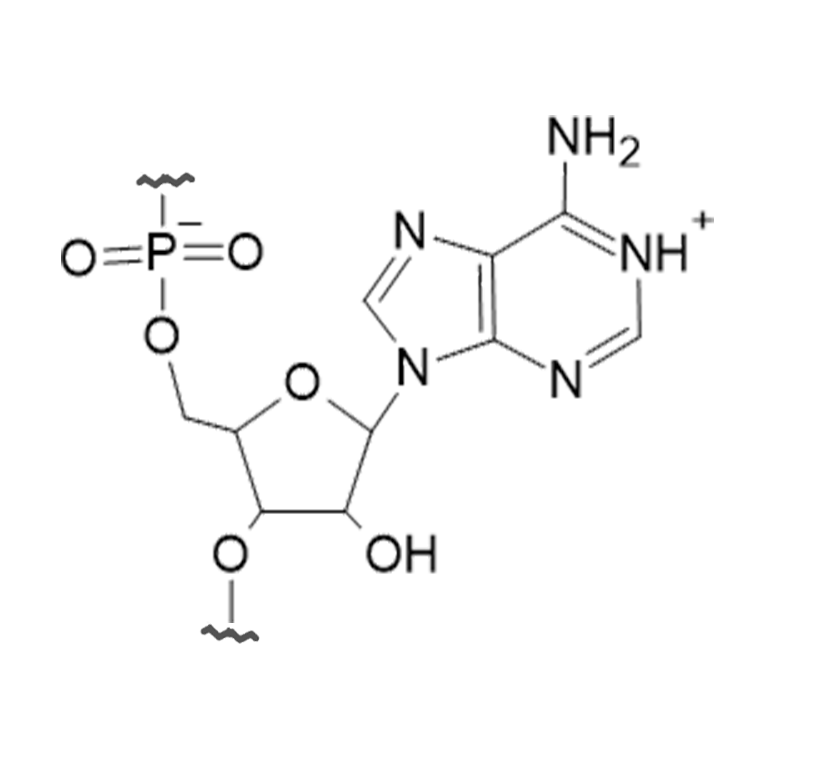
\includegraphics[width=30mm]{figures/chap3/RAP_cut.png}}{} & RAP & A38 & All & 0 & available in \cite{mlynsky_extensive_2010} \\
\subf{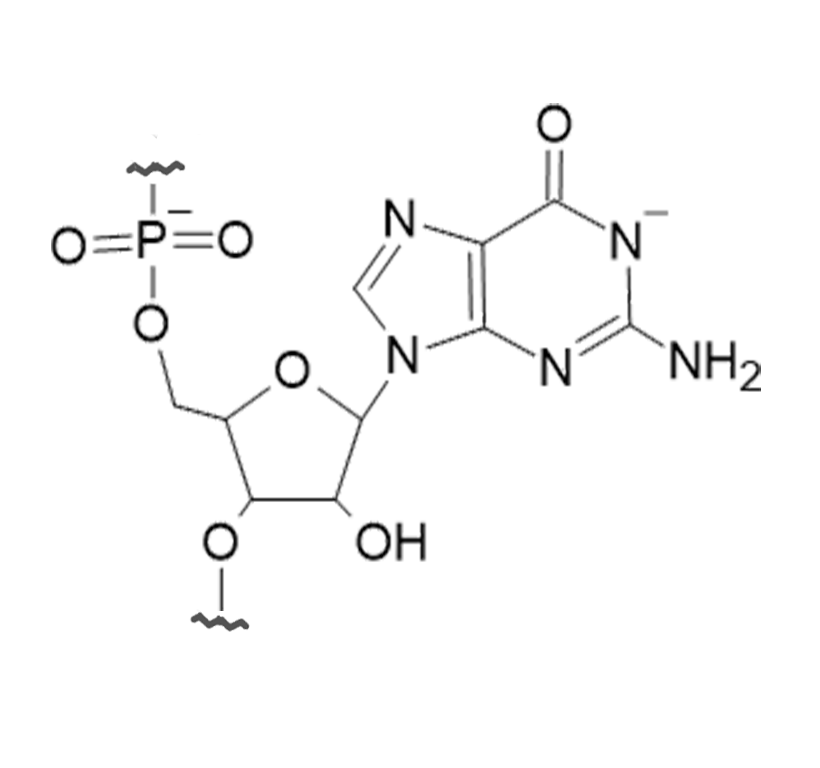
\includegraphics[width=30mm]{figures/chap3/RGM_cut.png}}{} & RGM & G8 & Dianionic & -2 & adapted from \cite{mlynsky_extensive_2010} \\
\subf{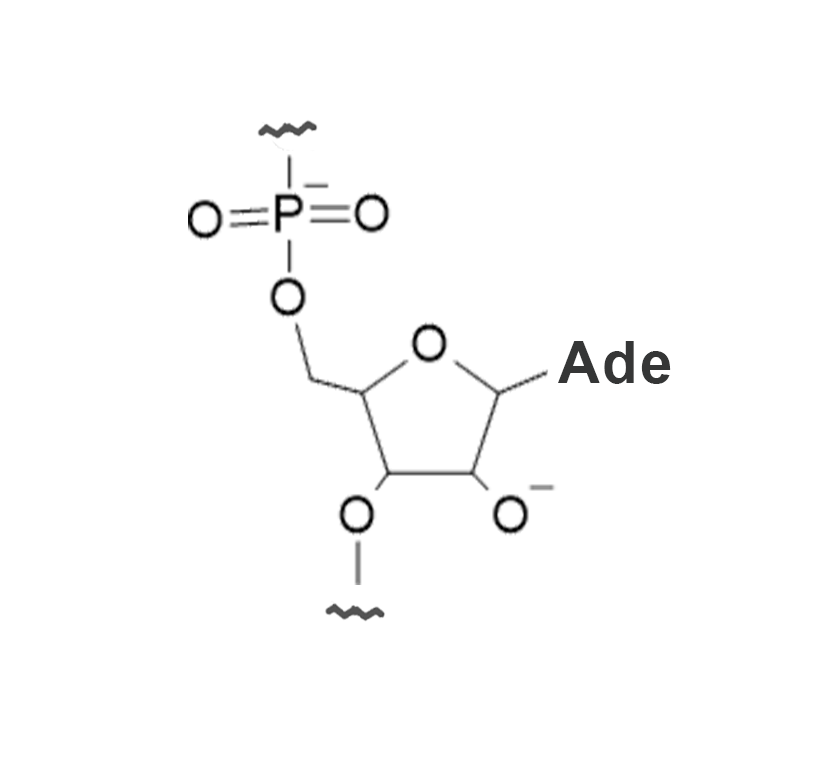
\includegraphics[width=30mm]{figures/chap3/AD_cut.png}}{} & AD  & A-1 & Dianionic & -2 & / \\
\subf{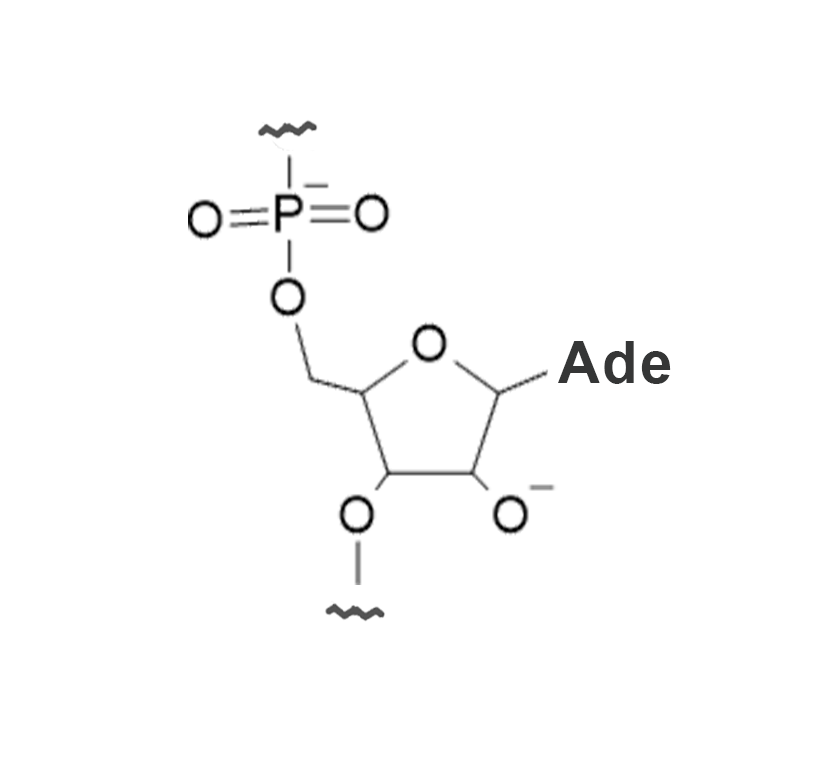
\includegraphics[width=30mm]{figures/chap3/RAA_cut.png}}{} & RAA & A-1 & Mono-anionic & -2 & adapted from \cite{kumar_mechanistic_2018} \\
\subf{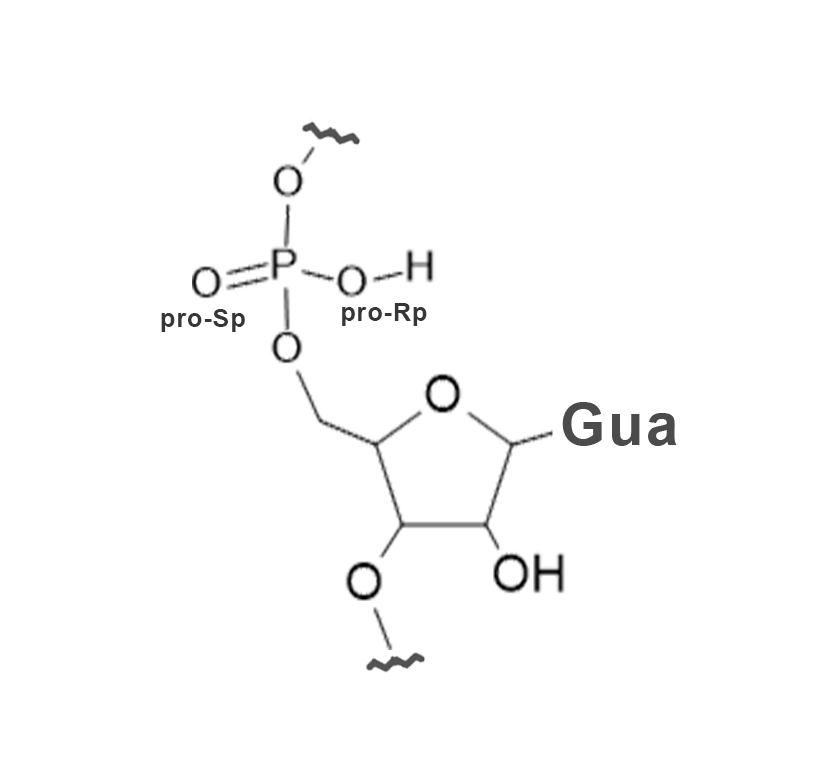
\includegraphics[width=30mm]{figures/chap3/GAA_cut.png}}{} & GAA & G+1 & Mono-anionic & 0 & adapted from \cite{kumar_mechanistic_2018} \\
\subf{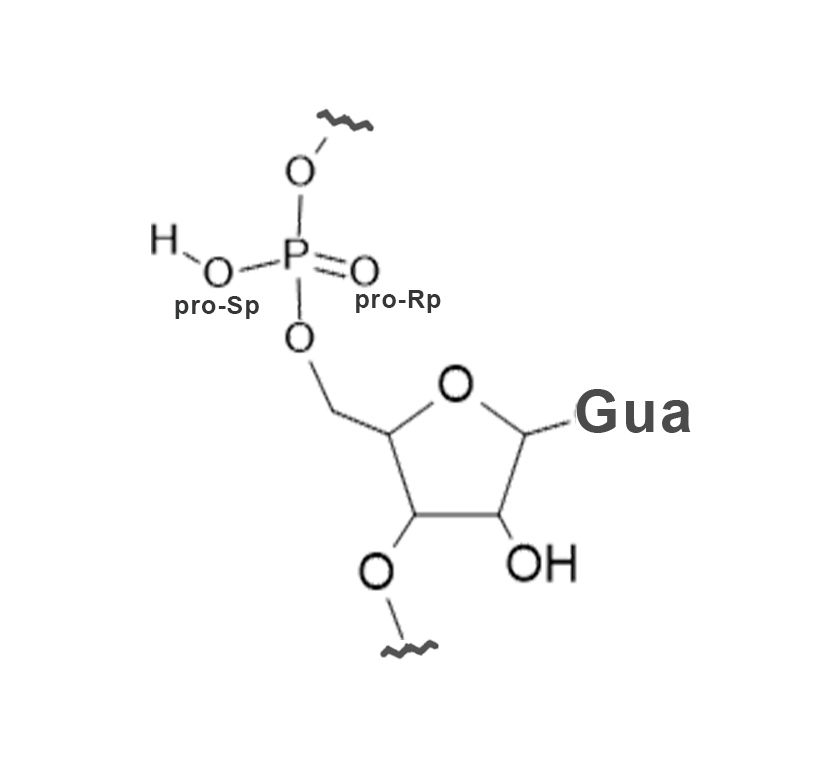
\includegraphics[width=30mm]{figures/chap3/GSA_cut.png}}{} & GSA & G+1 & Mono-anionic & 0 & adapted from \cite{kumar_mechanistic_2018} \\
\subf{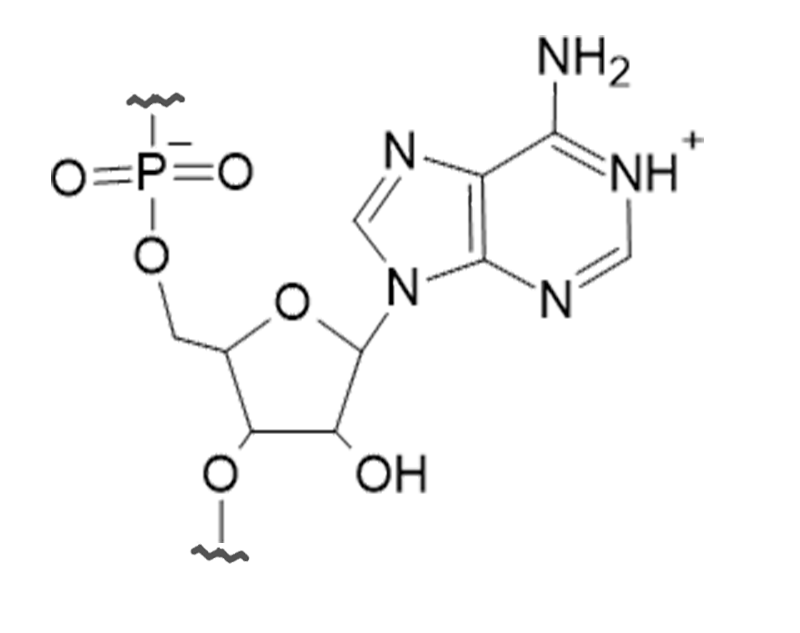
\includegraphics[width=30mm]{figures/chap3/RAP_clean.png}}{} & RAC & A-1 & All & -1 & / \\

\end{tabular}
\end{scriptsize}
\end{table}

\end{suppinfo}

%%%%%%%%%%%%%%%%%%%%%%%%%%%%%%%%%%%%%%%%%%%%%%%%%%%%%%%%%%%%%%%%%%%%%
%% The appropriate \bibliography command should be placed here.
%% Notice that the class file automatically sets \bibliographystyle
%% and also names the section correctly.
%%%%%%%%%%%%%%%%%%%%%%%%%%%%%%%%%%%%%%%%%%%%%%%%%%%%%%%%%%%%%%%%%%%%%
\bibliography{achemso-demo}

\end{document}